\documentclass[conference]{IEEEtran}
\IEEEoverridecommandlockouts
% The preceding line is only needed to identify funding in the first footnote. If that is unneeded, please comment it out.
\usepackage{cite}
\usepackage{bm}
\usepackage{amsmath,amssymb,amsfonts}
\usepackage{algorithm} 
\usepackage{titlesec}
\usepackage{algpseudocode}
\usepackage{graphicx}
\usepackage{mdframed}
\usepackage{enumerate}
\usepackage{textcomp}
\usepackage{xcolor}
\usepackage{svg}
\usepackage{tabularx,booktabs}
\usepackage{caption}
\usepackage{xcolor}
\usepackage{subcaption}

\newcolumntype{C}{>{\centering\arraybackslash}X} 
\setlength{\extrarowheight}{1pt} % for a bit more open "look"
\usepackage{lipsum} % filler text

\newcommand{\name}{TraDWin}

% Redefine the format for subsection numbering
\renewcommand{\thesubsection}{\arabic{subsection}.}

% Redefine the format for subsubsection numbering
\renewcommand{\thesubsubsection}{(\roman{subsubsection})}

% Adjust the formatting of subsection titles to be bold
\usepackage{titlesec}
\titleformat{\subsection}{\bfseries}{\thesubsection}{1em}{}

% Adjust the formatting of subsubsection titles to be bold
\titleformat{\subsubsection}{\bfseries}{\thesubsubsection}{1em}{}

\def\BibTeX{{\rm B\kern-.05em{\sc i\kern-.025em b}\kern-.08em
    T\kern-.1667em\lower.7ex\hbox{E}\kern-.125emX}}
\begin{document}



\title{\name: An interactive Digital Twin for City Traffic}

\author{
    \IEEEauthorblockN{Shreyansh Yadav}
    \IEEEauthorblockA{\textit{Department of Computer Science Engineering} \\
    \textit{IIT BHU, Varanasi}\\
    India \\
    shreyansh.yadav.cse19@itbhu.ac.in}
    \and
    \IEEEauthorblockN{Dr. Vignesh Sivaraman}
    \IEEEauthorblockA{\textit{Assistant Professor} \\
    \textit{Department of Computer Science and Engineering} \\
    \textit{IIT BHU, Varanasi}\\
    India \\
    vignesh.cse@iitbhu.ac.in}
}

\maketitle

\begin{abstract}
In the current era marked by rapid urbanization and population growth, cities worldwide face new challenges, chief among them being the effective management of traffic congestion and the optimization of transportation infrastructure. With reliable real-time data available through the emerging potential of smart cities powered by 5G and the Internet of Things (IoT), the use of sophisticated cyberphysical systems like Digital Twins is becoming increasingly viable. Such systems, powered by the ready availability of large amounts of data and machine learning methods, can prove to be increasingly effective at modeling the dynamics of urban traffic flow in real-time.

In this paper, we present \name, which is a Traffic Digital Twin (TDT) designed to seamlessly aggregate streaming traffic data from a myriad of sources, including traffic sensors, cameras, GPS devices, and more. Through the integration of physics-informed deep machine learning models, our model serves as an alternative to traditional empirical methods of slow and resource-intensive large-scale micro-simulations. By incorporating road network information, traffic volumes at different points, and other semantic information such as road characteristics and weather, the interactive TDT is designed and tested for three crucial aspects related to urban traffic state estimation: (i) prediction of future traffic states (ii) imputation of traffic state information on missing links, and (iii) traffic re-assignment on changing map topology, which can be useful for scenarios such as road closures or new construction planning. We test and validate our model using traffic volume data across Dublin city obtained from the SCATS traffic management system and also through SUMO-based micro-simulations of relevant scenarios.

\end{abstract}

\begin{IEEEkeywords}
Digital Twins, Traffic, Traffic state estimation, Traffic imputation, Traffic prediction, Urban Planning, Physics Informed Model
\end{IEEEkeywords}

\section{Introduction}
Today's rapid urbanization underscores the critical challenge of optimizing traffic and planning city infrastructure around it. Numerous studies have explored the direct and indirect impacts of traffic on health\cite{levy2010evaluation}, financial\cite{gorea2016financial}, and social domains\cite{anciaes2017social}. Hence, research into intelligent systems that can assist in this direction is imperative.

The Digital Twin, as a recent development within cyber-physical systems (CPS), has garnered increased attention in recent decades\cite{guo2017mobile}\cite{singh2021digital}, particularly today with the advancements in big data, IoT connectivity, and affordable computing, which make such systems increasingly practical today. A Digital Twin is a virtual representation of a real-world object\cite{VANDERHORN2021113524}, system, or process meticulously designed to replicate its physical counterpart in the digital realm. This allows it to capture and simulate the intricate details of a physical entity, enabling real-time monitoring, analysis, and prediction of its behavior. It goes beyond mere 3D modeling by incorporating live data, sensor inputs, and advanced analytics, providing a dynamic and interactive digital mirror of the physical world\cite{VANDERHORN2021113524}. This capability has found applications across a multitude of fields, from manufacturing and engineering to healthcare, urban planning, and beyond.

Our traffic digital twin, \name, as referred to in this paper, is an interactive simulation of city traffic that continuously updates its internal state with real-time traffic data from various sources. With the rise of smart cities equipped with IoT sensors and live camera feeds, there are numerous existing methods and theoretical approaches to enhance this capability. For instance, the Sydney Coordinated Adaptive Traffic System (SCATS)\cite{scats}, initially developed in Australia, utilizes inductive loop-based sensors at traffic signals to monitor traffic volume. It's already operational in over 180 cities across 28 countries, including New Zealand, Dublin, Shanghai, and Hong Kong \cite{wiki:sydney_traffic_system}. Similarly, cities like New York and Los Angeles have devised their own systems similar to SCATS. Other approximate techniques involve traffic probes\cite{zhu2012probe}, mobile phones with GPS\cite{rose2006mobile}—exemplified by Google's provision of congestion and travel time data—and the use of deep learning computer vision models with cameras to identify and count vehicles passing through roads. However, it's important to note that these methods primarily provide absolute volume count numbers at different nodes, as compared to collecting more granular data, such as source-destination pairs, which poses logistical and privacy challenges. In our study, we rely solely on absolute traffic volume data without other information related to individual vehicles.

In our paper, we aim to provide an end-to-end framework for the challenges of real-time data collection and aggregation. Along with a model that aims to solve three key tasks related to traffic modeling, which are as follows:
\begin{enumerate}[(i)]
    \item \textit{Traffic Prediction:} Given a traffic volume time series, our goal is to forecast future values, essentially predicting future dynamics based on historical data.
    
    \item \textit{Imputation:} Given a traffic volume time series with missing data, which could be due to sensor failure, etc., fill in the missing values as accurately as possible.
    
    \item \textit{Re-assignment on edge addition or removal:} Predicting how traffic flow will be affected by changes in the road network, such as adding or removing a road segment.
\end{enumerate}

In the contemporary literature review, as we discuss later, we see mathematical as well as deep learning time series analysis methods are prevalent for tasks (i) and (ii). However, for the task (iii), microscopic traffic simulation software like SUMO\cite{sumo} and Vissim\cite{vissim} are commonly employed. Such simulation engines are resource-intensive and require comprehensive information on vehicle types, sources, and destinations to yield accurate results, which may not be easily collected. Another general limitation of previous approaches, that focus only on time series analysis, is that all computation is done only taking into account traffic flow data, ignoring any possible exogenous variables like weather\cite{weather}, holidays\cite{holiday}, etc.

In our research, we assert that traffic dynamics are influenced not only by intrinsic relations within the data but also by extrinsic factors\cite{weather}\cite{holiday}, and hidden relationships may exist among these features, which are not immediately apparent. Thus, the TDT model we propose is very easily extensible and includes new features that extend model prediction capabilities.

For the model, we use an informed Wasserstein distance-based GAIN, which is a modified Generative Adversarial Imputation Net (GAIN)\cite{gain} (a class of conditional GANs) with modifications from Wasserstein GAN (WGAN)\cite{wgan} which have been shown to be very effective in training GANs\cite{wgan}. It also includes a modified loss function from physics-informed deep learning techniques\cite{pidl}, which helps the model to conform to the physical laws of conservation. 

We use Node2Vec\cite{node2vec} to convert graph nodes to feature embeddings representing their structure and then append relevant traffic data and other semantic information like weather after encoding them using Word2Vec\cite{word2vec} to the embeddings. 

We train and test our model on real-world traffic data obtained from the SCATS\cite{scats} system in Dublin city and also on specific scenarios generated and simulated in SUMO\cite{sumo} (Simulation of Urban Mobility) simulations.

Finally, we summarise the contributions of our study as follows:
\begin{enumerate}[(i)]
  \item Proposing an end-to-end workflow of an interactive Traffic Digital Twin system with traffic volume data as input.
  \item Developing and testing a new physics-informed Wasserstein distance-based GAIN model to predict and model different tasks on real-world Dublin city traffic data.
  \item Exploring physics-informed models to effectively model physical phenomena related to traffic modeling.
\end{enumerate}

Section I introduces our work, and Section II explores the existing research related to our work. Section III explains the methods used along with the details of the implementation to replicate the model. It also compares our approach with the existing work in this direction. Section IV presents the experiment details and the results of the proposed methods, and finally, Section V concludes the report.

\section{Related Work}

In this section, we briefly go over the existing work done related to traffic modeling, primarily existing spatiotemporal modeling methods, both deep learning and mathematical, and compare them with our approach. We address contemporary work done for each of the different tasks that the model aims to perform, i.e., prediction, imputation, and prediction on changing topology, which is unique to our paper.

Autoregressive Integrated Moving Average (ARIMA) \cite{arima} and its variants, such as time-oriented ARIMA\cite{time_arima} and Seasonal ARIMA\cite{sarima}, are extensively employed traditional algorithms for prediction and forecasting tasks. ARIMA operates on time series data and is often combined with other algorithms to incorporate spatial features. For example, C. Xu et al. (cite) integrated ARIMA with a genetic algorithm to estimate upcoming traffic flow on roads. While ARIMA models are adept at capturing linear time series data, the addition of genetic algorithms enhances their capability to extract features from nonlinear historical data. This integration underscores the versatility and adaptability of ARIMA-based approaches in addressing complex prediction challenges. Hence, we also compare our model performance with the ARIMA model.

Other methods like Temporal Regularized Matrix Factorization (TRMF)\cite{trmf}, Bayesian Temporal Regularized Matrix Factorization (BTRMF)\cite{btrmf}, Bayesian Temporal Matrix Factorization and (BTMF)\cite{btrmf} have also been explored in the context of traffic prediction. These methods extend the principles of matrix factorization and tensor factorization to capture temporal dependencies and spatial correlations in high-dimensional traffic data. TRMF\cite{trmf}, introduced by Lai et al. (2017), extends TRMF to tensor data structures, allowing for the modeling of multi-dimensional traffic flow data with enhanced flexibility. Similarly, BTRMF\cite{btrmf}, proposed by Liu et al. (2019), integrates Bayesian inference into tensor factorization to provide probabilistic predictions and uncertainty quantification in traffic forecasting tasks. On the other hand, BTMF and BTTF extend the Bayesian framework to matrix and tensor factorization, respectively, offering robust approaches for modeling temporal dynamics and spatial interactions in traffic networks while accounting for uncertainties in the prediction process. These methods contribute to the diverse landscape of predictive models for traffic prediction, each offering unique advantages and insights for tackling the challenges of forecasting traffic flow accurately.

Graph Neural Networks (GNNs)\cite{gnn} have emerged as a prominent tool for spatiotemporal modeling, demonstrating effectiveness in various applications such as traffic forecasting and imputation. For instance, studies by Li et al. (2018) and Zhang et al. (2019) have showcased their utility in accurately predicting traffic patterns and filling in missing data in traffic volume time series. GNNs operate by iteratively updating node representations based on their local neighborhood information, allowing them to capture complex spatial and temporal dependencies within graph-structured data. However, a limitation of traditional GNNs is their reliance on the static network topology during training, which poses challenges when adapting them to dynamic graphs. As a result, they may not be suitable for tasks involving changes in the graph structure, such as predicting traffic flow upon adding or removing edges, which is a crucial aspect of our research focus.

Physics-informed deep learning (PIDL)\cite{raissi2017physics} is an emerging deep learning methodology wherein a neural network undergoes training to tackle learning tasks while adhering to the principles of physics, as given by physics-based constraint equations, general nonlinear partial differential equations, etc. This way, the fundamental laws of physics are ingrained as a bias during training, and the model does not have to figure out those dependencies on its own, which allows the resultant neural network to be data-efficient.

For traffic modeling, PIDL serves as an effective middle ground between purely data-driven models and purely model-driven methods. Purely model-driven approaches use a set of mathematical models and prior knowledge of traffic dynamics as input to estimate future states. They assume the model to be an accurate representation of real-world traffic; however, such an assumption fails to capture the intricate dynamics of real-world traffic. Moreover, different equally viable models exist for the same task, and while one may be better than another for specific data, generalization across models is hard. Some examples of model-driven traffic approaches are the Lighthill-Whitham-Richards (LWR)\cite{lwr} model, the Cell Transmission model (CTM)\cite{ctm}, etc. In contrast, pure deep learning approaches require large amounts of data in order to learn a good generalized relation since they learn without any pre-existing information on physical relations and constraints. Hence, physics-informed deep learning combines both approaches by trying to bias the deep learning model to learn the physics-based results using some parameter $\lambda$ while still allowing enough freedom to learn more granular relations in traffic dynamics.

\section{Methodology}

\subsection{\textbf{Problem Statement}}

A road network can be considered an undirected graph $G = (V, E)$ where $V$ represents nodes, which is a collection of $N$ detector nodes, i.e., $V=\{v_1,v_2,...,v_n\}$ where $N = |V|$ and $v_i$ is the $i$th detector node. $E$ represents the $N_E = |E|$ road links connecting the detectors, and let $A \in \mathbb{R}^{N \times N}$ denote the adjacency matrix of $G$, i.e., $A = \{e_{ij}\}, i,j=1$ to $N$ where $e_{ij} = 1$ if nodes $v_i$ and $v_j$ are adjacent and $0$ otherwise.

Let each node of graph $G$ at time $t$ be represented by a $D$-dimensional feature vector represented as $\mathbf{x}_i^t \in \mathbb{R}^D$ that represents the node embeddings generated as explained later using node embeddings obtained from Node2Vec, other meta-information encoded, and traffic volume counts. Also, let the volume of traffic at time $t$ at node $i$ be $c_i^t$.

Define feature vectors for all nodes at a particular time $t$ as
\begin{equation*}
    \mathbf{X}_t = (\mathbf{x}_1^t, \mathbf{x}_2^t, \ldots, \mathbf{x}_N^t) \in \mathbb{R}^{N \times D} \tag{1}
\end{equation*}
Let the number of timesteps denoted by $T$ be a hyperparameter denoting the number of consecutive time steps under consideration. Then denote the values of all feature vectors over all nodes over $T$ consecutive time intervals starting at some time $t_0$ as
\begin{equation}
    \bm{\chi} = (\mathbf{X}_{t_0}, \mathbf{X}_{t_0+1}, \ldots, \mathbf{X}_{t_0+T-1}) \in \mathbb{R}^{T \times N \times D} \tag{2}
\end{equation}

Given the aforementioned notation, the problem that we are tackling in this paper can be formally define as proposing as Traffic Digital Twin (TDT) that can perform the following tasks:
\begin{enumerate}[(i)]
    \item \textbf{Traffic prediction:} Given graph $G(V, E)$ and a sequence $\bm{\chi}$ of feature vectors of observed historical traffic flow over $T$ consecutive intervals, i.e., $\bm{\chi} = (\mathbf{X}_{t_0}, \mathbf{X}_{t_0+1}, \ldots, \mathbf{X}_{t_0+T-1})$, predict $\mathbf{Y}$, the traffic volume counts $c_i$ for $i \in N$ at the next timestep $t_0+T$, i.e., $\mathbf{Y} = \{c_1^{t_0+T}, c_2^{t_0+T}, \ldots, c_N^{t_0+T}\}$. Henceforth, we refer to this task as task (i).
    \item \textbf{Imputation:} Given graph $G(V,E)$ and a sequence $\bm{\chi}$ of feature vectors of observed historical traffic flow over $T$ consecutive intervals, i.e., $\bm{\chi} = (\mathbf{X}_{t_0}, \mathbf{X}_{t_0+1}, \ldots, \mathbf{X}_{t_0+T-1})$, a binary mask vector $\mathbf{M} \in \mathbb{R}^{N \times T}$ such that $\mathbf{M} = \{m_{ij}\}$ where $m_{ij} = 1$ if the traffic volume count at detector $i$ at time $t$ i.e. $c_{ij}$ is known and 0 otherwise to indicate its missing, impute the missing $c_{ij}$ values. Henceforth, we refer to this task as task (ii).
    \item \textbf{Traffic assignment on edge addition/removal:} Given original graph $G(V,E)$ and the new modified graph $G'(V', E')$ with an edge $e$ added or removed. Let $\phi$ be a hyperparameter denoting the number of closest neighbor nodes to the changed edge to mask out, i.e., $\mathbf{M} = \{m_i\}$ where $m_i = 1$ if the $\text{dist}(v_i,e)> \phi$ and 0 otherwise. Predict $\mathbf{Y'} = \{c'_1, c'_2, \ldots, c'_N \}$ where $c'_i$ is the traffic volume of the detectors with the modified topology $G'$. Henceforth, we refer to this task as task (iii).
\end{enumerate}

\subsection{\textbf{Data streaming framework}}

Reliable real-time data collection is a crucial aspect and prerequisite of a digital twin to effectively update internal parameters and synchronize with the real world. The Traffic Digital Twin (TDT), \name, presented in this paper requires real-time traffic volume data as input. We aim to use absolute traffic volume counts available at a manageable low frequency of 15 minutes to one hour. While systems with more sophisticated data at a higher frequency can be proposed, we aim to keep the real-world collection infrastructure cheap, simple, and based on already existing systems around the world. In particular, we strive to cater to the following objectives:

\begin{figure*}[t]
  \centering
  \includegraphics[width=0.77\textwidth]{framework.pdf} % Adjust width as needed
  \caption{Traffic Digital Twin (TDT) data processing}
  \label{fig:framework}
\end{figure*}

\begin{enumerate}[(i)]
    \item Hardware infrastructure should be cheap and easily replaceable.
    \item Easily extendable to use a variety of different sources.
    \item Should work with only absolute traffic counts, no other specific information like direction and vehicle types.
    \item Should work with a medium frequency update.
\end{enumerate}

There are various possible ways to collect the type of data mentioned. The most reliable would be to install inductive loop detectors embedded in road surfaces at city intersections. Such systems are already available and in use in several major cities. For example, the Sydney Coordinated Adaptive Traffic System (SCATS)\cite{scats} is available in over 180 cities across 28 countries, including New Zealand, Dublin, Shanghai, and Hong Kong \cite{wiki:sydney_traffic_system}. New York City's Adaptive Traffic Control System (ATCS), Adaptive Signal Control Technology (ASCT), SCOOT, and ACS are other such systems which are used to control traffic signal timings and optimize congestion. Such systems can be easily extended to use with our proposed model since we only use absolute traffic volume counts which such systems are capable of collecting.

Another possible data source can be surveillance cameras assisted with computer vision models\cite{jain2019review}. which is already used in practice at some intersections in Shenzhen, China. Several existing studies\cite{asha2018vehicle} using state-of-the-art object detection models like YOLO\cite{redmon2018yolov3} demonstrate effectiveness of this method. Such a model based approach allows for cheap and effective traffic monitoring on top of existing surveillance camera infrastructure. 

Other methods like using GPS-enabled mobile phones\cite{rose2006mobile} to track urban traffic flow, as Google does in its Maps product, and the use of probe vehicles\cite{zhu2012probe}, which are vehicles equipped with detectors that may be taxis or public transport, can also be used to approximate traffic volume based on their data.

We aim for our model to work in conjunction with multiple data streams, as that different parts of the road network may be served with different data sources. We want our TDT to seamlessly integrate with these sources, so we need an aggregator of sorts to reconcile the data from the different streams and store them in a data lake. This data can then be used by the TDT model to keep its internal state in sync with real-world data.

The deployed aggregator system will have an RPC and API interface can be interacted with by the remote sensors and other data sources. Each different service can have a separate interface build for interacting with the aggregator service. The aggregator then stores all the data with relevant meta information in a datalake which is a centralized repository that allows you to store all your structured and unstructured data. We make use of a datalake as different sources might have additional information apart from just traffic volume counts and we by allowing to store other complementary information we leave possible avenues for building up further capabilities in our TDT.

An example representing a simplied view of the aforementioned process is shown in Fig. \ref{fig:framework}.

\subsection{\textbf{Model input}}

For each node, we create a feature vector that represents all the information related to that node. The feature vector for a node is composed of three feature vectors that are as defined ahead, concatenated:

\subsubsection{Graph embedding generation using Node2Vec:}

In order for the model to effectively learn the spatial relationships between the detector nodes based on graph structure, we need a way to generate an appropriate representation of the graph nodes that capture the neighborhood structure effectively. $Node2Vec$\cite{node2vec} is a feature learning algorithm that uses second-order biased random walks in a Skip-gram architecture to learn feature vectors for nodes in the graph. There are two key steps for feature generation:

\begin{enumerate}[(i)]
    \item \textit{Sampling using second order biased random walks}: Two hyper-parameters \( p \) and \( q \) are introduced which are the "return" and "in-out" parameters respectively. Suppose we simulate a random walk of fixed length \( l \). Let \( c_i \) denote the \( i \)th node in the walk, starting with \( c_0 = u \). Nodes \( c_i \) are generated by the following distribution:
    \[
        P(c_i = x \mid c_{i-1} = v) =
        \begin{cases}
        \frac{\pi_{vx}}{Z} & \text{if } (v,x) \in E \\
        0 & \text{otherwise}
        \end{cases}
    \]
    where \( \pi_{vx} \) is the unnormalized transition probability between nodes \( v \) and \( x \), and \( Z \) is the normalizing constant.
    
    For a walk that just traversed edge \( (t,v) \) and now resides at node \( v \), we now needs to decide on the next step so it evaluates the transition probabilities \( \pi_{vx} \) on edges \( (v,x) \) leading from \( v \). The transition probability \( \pi_{vx} = \alpha_{pq}(t,x)\cdot w_{vx} \), where 
    \[
        \alpha_{pq}(t,x) = 
        \begin{cases}
        \frac{1}{p}  & \text{if } d_{tx} = 0\\
        1 & \text{if } d_{tx} = 1\\
        \frac{1}{q} & \text{if } d_{tx} = 2
        \end{cases}
    \]
    and \( d_{tx} \) denotes the shortest path distance between nodes \( t \) and \( x \).

    \item \textit{Optimizing objective function using Skip-gram}: Let for graph \( G(V, E) \), \( f: V \rightarrow \mathbb{R}^d \) be the \( d \)-dimensional feature representation function. Thus, \( f \) is a matrix of size \( |V| \times d \) parameters. Now let for every node \( u \in V \), we define \( N_S(u) \subset V \) as a \emph{network neighborhood} of node \( u \) generated in step (i). Define similarity between two nodes \( u \) and \( v \) as:
    \[
        P_f(v|u) = \frac{\exp(f(v)^T f(u))}{\sum_{w \in V} \exp(f(w)^T f(u))} \tag{1}
    \]
    For neighborhood \( N_s(v) \) of \( v \), define the probability of the neighborhood of \( u \) as:
    
    \[ P_f(N_s(u)|u) = \prod_{v \in N_s(u)} P_f(v|u) \tag{2} \]

    Further, the global neighborhood likelihood for a given \( f \) can be define as:
    \[ \sum_{u \in V} \log P_f(N_s(u)|u) \tag{3}\]
    which is the objective function that we want to maximize through out feature representation function \(f\). Hence,
     \[
    \max_{u \in V} \sum_{u \in V} \log \left( \prod_{v \in N_s(u)} \frac{\exp(f(v)^T f(u))}{\sum_{w \in V} \exp(f(w)^T f(u))} \right) \tag{4}
    \]
\end{enumerate}

\begin{figure*}[htbp]
  \centering
  \includegraphics[width=0.85\textwidth]{model.pdf}
  \caption{Model architecture}
  \label{fig:dataset}
\end{figure*}

\subsubsection{Traffic volume normalised:}
The input data should be normalised to increase the training speed and effectiveness. The traffic volume counts at different detectors is normalised as:
\[
x_{\text{norm}} = \frac{x - x_{\text{min}}}{x_{\text{max}} - x_{\text{min}}}
\]
Thus, \( x_{\text{norm}} \) is in the range \([0,1]\) after normalization. This same approach is used for other continuous or discrete single valued features.

\subsubsection{Word2Vec encoding of other exogeneous variables:}
Skip-gram\cite{skipgram}, a popular Word2Vec\cite{word2vec} architecture, aims to predict the context words given a target word. It learns to encode the semantic meaning of words by maximizing the probability of context words given the target word. Mathematically, the objective function for Skip-gram can be represented as:

\[
J_\theta = \frac{1}{T}\sum^{T}_{t=1}\sum_{-n\leq j \leq n, j \neq 0}\log p\left(w_{j+1} \mid w_{t}\right)
\]

where \( w_t \) represents the target word at position \( t \), \( c \) is the size of the context window, and \( T \) is the total number of words in the corpus.

We use \textit{Word2Vec} to encode the other possibly relevant exogenous variables like weather, road-type etc. as features to the model input, thus increasing its effectiveness. We would like to note that this approach is easily extensible to any number of other features that may prove to be relevant in the future, and we wish to add to the model input.

\vspace{3ex} Concatenating the feature vectors from above sub-parts, we get the final input vector. Extending the notation as define in section III.A, for \(N\) nodes, we define the construction of \(\mathbf{x}_i^t\), the feature vector of node \(i\) at time \(t\). Assuming \textit{Node2Vec} was used as defined in (i), to generate \(R^{D_g}\) dimensional graph embeddings for each node. Let \(g_i\) be the graph embedding for node \(i\). Then, for \(n\) single-dimensional real-valued features \((r_1, r_2, \ldots, r_n)\), let them be normalized as defined in (ii) to \((r_1^{\text{norm}}, r_2^{\text{norm}}, \ldots, r_n^{\text{norm}})\) thus creating a \(D_n = n\) dimensional vector. Let them be represented by \(h_i^t\). Finally, for \(m\) "words" representing other semantic information related to the node, and using \textit{Word2Vec} to output \(d_w\) dimensional vectors for each word, we get a \(R^{mxd_w}\) dimensioned vector that we flatten and represent as \(k_i^t\) \(\in\) \(R^{D_w}\) where \(D_w = m \times d_w\).

Finally, one concatenation of the above three, we get the feature vector of node \(i\) at time \(t\) 
\[\mathbf{x}_i^t = (\ g_i\ ||\ h_i^t\ ||\ k_i^t\ ) \in R^D\] 
where \(D = D_g+D_n+D_w\).
Thus, from (i) and (ii), over \( T \) consecutive time steps and for \( N \) nodes, we get the final feature vector as \( \mathbf{\chi} \)  \(\in\) \( \mathbb{R}^{T \times N \times D} \).
Depending on the task, we also add other task-specific inputs like for the case of imputation a binary matrix \( M \) representing the missing and known values. Specific implementation details are discussed further in the experiments section.

\subsection{\textbf{Physics Informed Deep Learning}}

Physics-informed deep learning (PIDL) represents a distinct approach within deep learning (DL), where a neural network is trained to tackle learning tasks while adhering to the principles of physics. By integrating fundamental physical laws as prior knowledge, the resulting neural network serves as a data-efficient approximator, adept at processing input data and delivering accurate predictions.

In situations where systems are required to adhere to the physical laws, PIDL is specially useful as it biases the model to follow the physics models, this allows the model to generate more accurate results, specially GANs as this eliminates several possible predicted distributions that are not viable do to not adhering to the physical laws of the system.

In our situation, specifically with problem 3. of Traffic assignment on edge addition/removal, where we have to predict the changed volume counts on the same timestep but with modified topology, it is imperative, according to the \textit{conservation law} of traffic, that in such a case that the total volume of traffic in a large enough region prior to and after redistribution will be same.

Formally, for a particular fixed time, let \( G(V,E) \) be the original graph, and \( G'(V',E') \) be the graph obtained by adding or removing an edge \( e \). Similarly, \( c_i \) represents the traffic volume at detector \( i \) in \( G \) for \( i = 1 \) to \( N = |V| \), and \( c_i' \) represents the traffic volume at detector \( i \) in \( G' \) for \( i = 1 \) to \( N' = |V'| \). Then from \textit{conservation law}:
\begin{equation}
    C = \sum_{i=1}^{N} c_i = C' = \sum_{i=1}^{N'} c'_i \tag{5}
\end{equation}

In order to bias the model for conservation as described in Eq. (3), it needs to be integrated into the learning process of the PIDL network. The simplest way to do it is to define it as an additional term to the loss used to update the model, basically penalizing the model heavily for predictions that do not conform to the physical constraints. With traffic volumes \(c_i\) along with other graph information as training input, we establish two different measures for the discriminator to evaluate generator output:
\begin{enumerate}
    \item \textbf{\( \mathcal{L}_{DL} \)}: Denoting the conventional discriminator loss defined as:
    \[ \mathcal{L}_{DL} = \mathbb{E}_{x \sim P_{\text{data}}}[D(x)] - \mathbb{E}_{z \sim P_z}[D(G(z))] \]

    \item \textbf{\( \mathcal{L}_{PHY} \)}: Denoting the conservation loss. As defined in Eq. (3), for a given mask \( M \), let \( S \) be the set of detectors such that \( M(i) = 0 \), specifically \( S = \{i \mid M(i) = 0\} \). Then let \( C_0 \) be the sum of masked traffic volume counts, i.e., \( C_0 = \sum_{i \in S} c_i \), and \( Y = \{c'_i \mid i \in S\} \) be the generator output. Then define:
    \[ \mathcal{L}_{PHY} = (C_0 - \sum_{i \in S} c'_i)^2 \]
\end{enumerate}
In order to control the dominance of the different components of the loss function, we introduce two new hyperparameters, \( \mu \) and \( \lambda \), to adjust the weights of \( \mathcal{L}_{DL} \) and \( \mathcal{L}_{PH} \) respectively. Thus, the final loss function can be defined as:

\[ \mathcal{L} = \mu \cdot \mathcal{L}_{DL} + \lambda \cdot \mathcal{L}_{PHY} \]

In conclusion, by leveraging hyperparameters, we can fine-tune the model's balance between different objectives. Biasing the discriminator to respect physical laws allows the generator to better capture underlying patterns in the data, a capability we found useful in our experiments as we describe ahead.

\subsection{\name: Traffic Model}

In this section, we present the architecture of our \name model, which is inspired from architectures of Generative Adversarial Imputation Nets (GAIN)\cite{gain} and Wasserstein Generative Adversarial Network (WGAN)\cite{wgan}. GAIN is a new and popular type of conditional GAN that has been applied to a variety of missing value imputation tasks on different datasets with favorable results. WGAN is an improvement over traditional GANs proposed by M. Arjovsky et al., that is designed to improve training stability by focusing on using Wasserstein distance metric instead of the traditional Jensen-Shannon divergence, along with some other architecture changes like gradient clipping, removal of sigmoid, etc., that have been shown to result in more reliable convergence and better quality samples.

\subsubsection{\textit{Generator:}}

The generator \( G \) accepts inputs of observed data, with missing values, denoted by \( \mathbf{X} \), the binary mask vector \( \mathbf{M} \) which indicates what are the missing values, and a noise vector denoted by \( \mathbf{Z} \). It produces imputed data \( \mathbf{X}_g \), representing a vector of imputations, which is then projected to form the complete imputed output \( \mathbf{Y}_0 \). 

Formally, the output of the generator \( G \) can be denoted as: 
\[ \mathbf{X}_g = G(\mathbf{X}, \mathbf{M}, (\mathbf{1}-\mathbf{M}) \odot \mathbf{Z}) \]

where \( \odot \) denotes the Hadamard product or the element-wise multiplication and \( \mathbf{Z} \) is the \( d \)-dimensional noise vector. \( \mathbf{X}_g \) represents the missing values which are then filled back in \( \mathbf{X} \) as per the mask \( \mathbf{M} \), and this makes the final generator output that is then passed off to the discriminator to judge.

\subsubsection{\textit{Discriminator:}}

Similar to the discriminator in traditional GANs, we also use another model called the Discriminator, denoted by \( D \), that acts as an adversary to the Generator \( G \) and trains it. The discriminator \( D \) defined in the original GAIN implementation as \( D : \mathbf{\chi} \rightarrow [0,1]^d \), outputs a binary vector instead of a single real value, which denotes what components of the generator input are real (observed) and what are fake (imputed). 

So, in contrast to the traditional discriminator as used in GANs, which predicts whether the generated result is entirely fake or real, the discriminator in GAIN predicts what components are real or fake. And the loss which is then used in SGD is the mean of losses for individual components.

\subsubsection{\textit{Hint}}
GAIN introduces a new concept called the hint mechanism, represented by a random variable \( \mathbf{H} \) taking values in a space \( \mathcal{H} \). The aim of this hint mechanism is to provide additional missing information to the discriminator about the mask. The following proposition was introduced and proved in the GAIN\cite{gain} original paper:

\begin{mdframed}[linewidth=0.5pt]
\textit{
\newtheorem{proposition}{Proposition}
\begin{proposition} \label{prop:nonunique}
    There exist distributions of \( \mathbf{X} \), \( \mathbf{M} \), and \( \mathbf{H} \) for which solutions to \( \hat{p}(\mathbf{x} | \mathbf{h}, m_i = t) = \hat{p}(\mathbf{x} | \mathbf{h}) \) for each \( i \in \{1, \ldots, d\} \), \( \mathbf{x} \in \mathcal{X} \), and \( \mathbf{h} \in \mathcal{H} \) such that \( p_h(\mathbf{h} | m_i = t) > 0 \) are not unique under the optimality criterion of GAN.
\end{proposition}
}
\end{mdframed}

This means that there may exist several possible distributions that \( G \) may generate that may seem valid to \( D \), so \( \mathbf{H} \) must provide enough information to uniquely identify the correct representation of the underlying data, which is what the hint mechanism aims to do.

The hint mechanism depends on the binary mask vector \( \mathbf{M} \), and for each imputed sample \( (\hat{\mathbf{x}}, \mathbf{m}) \), we draw \( \mathbf{h} \) from the distribution \( \mathbf{H} | \mathbf{M} = \mathbf{m} \). We then add \( \mathbf{h} \) as an extra input to the discriminator, resulting in a function \( D: \mathcal{X} \times \mathcal{H} \rightarrow [0, 1]^d \), where each component of \( D(\hat{\mathbf{x}}, \mathbf{h}) \) represents the probability that the corresponding component of \( \hat{\mathbf{x}} \) was observed given \( \hat{\mathbf{X}} = \hat{\mathbf{x}} \) and \( \mathbf{H} = \mathbf{h} \).
By varying how \( \mathbf{H} \) is defined, we control the level of information it provides about \( \mathbf{M} \).

\textcolor{gray!80}{\vrule width 0.95\columnwidth height 0.001pt depth 0pt \relax}

\vspace{1ex}

Finally, we take inspiration from the architecture of WGAN and incorporate some of those changes in our model. Traditional GANs suffer from training instability and model collapse, i.e., inability to learn the diverse representations and only generating repetitive samples. Wasserstein GAN (WGAN) proposed by M Arjovsky et. al, solves these problems and we highlight some of the architectural changes we made to GAIN based on WGAN in the following paragraphs.

In traditional GAN the generator and discriminator are trained using the following loss functions:
\[
\mathcal{L}_{\text{GAN}}^G = \log(1 - D(G(z)))
\]
\[
\mathcal{L}_{\text{GAN}}^D = -\log(D(x)) - \log(1 - D(G(z)))
\]

whereas in WGANs, we remove the logarithms and use Wasserstein distance for loss instead.
\[
\mathcal{L}_{\text{WGAN}}^G = -D(G(z))
\]
\[
\mathcal{L}_{\text{WGAN}}^D = D(G(z)) - D(x)
\]

Another change in WGANs, that we incorporate in GAIN is the absence of a sigmoid activation function in the discriminator's output layer, unlike in traditional GANs. This alteration enables the discriminator to output unbounded real-valued scores instead of probabilities. Additionally, WGANs incorporate gradient clipping as a regularization technique to enhance training stability. Gradient clipping involves setting a threshold value for the gradients, and if they exceed this threshold, they are scaled down to ensure that their magnitude does not surpass it. This approach helps stabilize the training process and mitigates issues such as exploding gradients.

\section{Experiments}

In this section we describe the experimental results of our model along with the necessary parameters required to reproduce those results. We also describe baselines that we compare our model with, along with their parameters.

\subsection{Dataset Description}

We use the real world traffic volumes of Dublin city streets collected using the SCATS (Sydney Coordinated Adaptive Traffic System)\cite{scats} system over a three month period. The SCATS system is used in Dublin as an adaptive urban traffic management system that synchronises traffic signals and optimises traffic flow across the entire city.

The dataset consists of traffic volumes from the 825 sensors at all key intersections in Dublin city, sampled at a frequency of 1 hour, during a time period of 3 months, from October 1, 2023 to December 31, 2023. The dataset contains the latitudinal and longitudinal geographical coordinates along with timestamped total volume of traffic detected by each detector in the one hour period.

We also verify the model for task (iii) on SUMO\cite{sumo} TAPASCologne scenario\cite{tapas}, which is a simulation configuration that describes the traffic dynamics of Cologne city in Germany for a day. The scenario is publicly available on the official SUMO website and was created using mobility demand data based on information about travelling habits of citizens and on information about the infrastructure of the area they live in. Since this testing is manual, we run a limited number of tests, where we change an edge and process the simulation, based on the default minimal travel time routing before and after the change, and observe the deviation between simulation and our results.

\begin{figure}[htbp]
  \centering
  \includegraphics[width=0.5\textwidth]{dataset.png}
  \caption{Snapshot of sensor locations plotted along with road network from Overpass API}
  \label{fig:dataset}
\end{figure}


\subsection{Model Parameters}

For all experiments, we set hyperparameters $T = 3$, which is the number of consecutive timesteps to consider for prediction and imputation tasks. For all tasks, we optimize the model input by assuming the locality of traffic within such a timespan and that any changes to a particular node are only dependent on nodes "close" to it. Formally, during training, we train on sub-graphs consisting of the node clusters instead of the entire graph all at once. Specifically, a subgraph is generated by choosing a node $u$ at random and then selecting all nodes that are at a distance less than $\sigma$ to it, specifically for $G(V,E)$, $G_{\text{sub}} = G\{v \in V \; | \; \text{dist}(u, v) < \sigma\}$. For our experiments, we set $\sigma$ as $2.5\ km$, which is a reasonable expectation as clusters usually contain 20 to 30 nodes within this range.

After sampling as stated before, we use a 80-20 test-train split, i.e., the model is trained on 80\% of the samples and then performance is verified on new unseen data that comprises of 20\% of the samples. The data is then modified based on the task at hand. For imputation, we followed MCAR (Missing Completely at Random) distribution and randomly masked values both spatially and temporally, following a parameter defined as the miss rate, we test our model on miss rates of 10\%, 20\%, 30\%, and 40\%. For prediction we, use the full data of three timesteps to predict the fourth step, by basically masking the values along the last timestep dimension. For re-assignment task, i.e., task (iii), we only consider one timestep and re-assign values for that same timestep but with modified spatial geometry.

\subsection{Baselines}

We compare our \name model with a number of different existing approaches across different domains including different mathematical analysis and deep learning techniques used popularly for these tasks.

One of the simplest approaches for imputation is \textit{KNN}. Similarly, for prediction, \textit{ARIMA}\cite{arima} stands for AutoRegressive Integrated Moving Average is used. Matrix factorization methods like \textit{TRMF}\cite{trmf} (Temporal Regularized Matrix Factorization) use latent factors for predictions, and its modification \textit{BTRMF}\cite{btrmf} (Bayesian Temporal Regularized Matrix Factorization) extends TRMF with a Bayesian framework. For both these methods, we use rank $= 10$, $1000$ burn-in iterations, and $200$ Gibbs iterations.

\textit{LRTC-TNN}\cite{lrtc} (Low-Rank Tensor Completion with Truncated Nuclear Norm) is a method for tensor completion. It uses parameters $\rho = 1e-5$, $\theta = 0.25$, and $\epsilon = 1e-4$. \textit{BGCP} (Bayesian Gaussian Process Factorization) is another method that utilizes Bayesian inference. For BGCP, we use similar burn-in and Gibbs iterations, and set rank $= 30$. It is worth noting that these model baselines are only applicable to task (i) and task (ii) and not for task (iii) since they were not built with that task as a consideration.

Finally, there are deep learning methods that we used. For imputation, we employed the \textit{Denoising AutoEncoder} (DAE)\cite{dae} model, which is effective in learning meaningful representations of the data while handling missing values. For prediction tasks, we utilized an \textit{LSTM}\cite{lstm} (Long Short-Term Memory) model as LSTM networks are well-suited for capturing temporal dependencies in sequential data.

\subsection{Evaluation metrics}

In order to evaluate the performance of the different methods and compare them, we use RMSE (Root Mean Squared Error) and MAPE (Mean Absolute Percentage Error). These metrics are defined as:


\[
\text{RMSE} = \sqrt{\frac{1}{n} \sum_{i=1}^{n} (y_i - \hat{y}_i)^2}
\]

\[
\text{MAPE} = \frac{1}{n} \sum_{i=1}^{n} \left| \frac{y_i - \hat{y}_i}{y_i} \right| \times 100\%
\]

where \( y_i \) represents the true value, \( \hat{y}_i \) represents the predicted value, and \( n \) is the number of samples.

\subsection{Results}

\begin{figure*}[]
    \centering
    \includegraphics[width=0.9\textwidth]{mape_pred.eps}
    \caption{MAPE on prediction task for different deltas (timesteps to predict ahead)}
    \label{fig:mape_pred}
\end{figure*}

\begin{figure*}[]
    \centering
    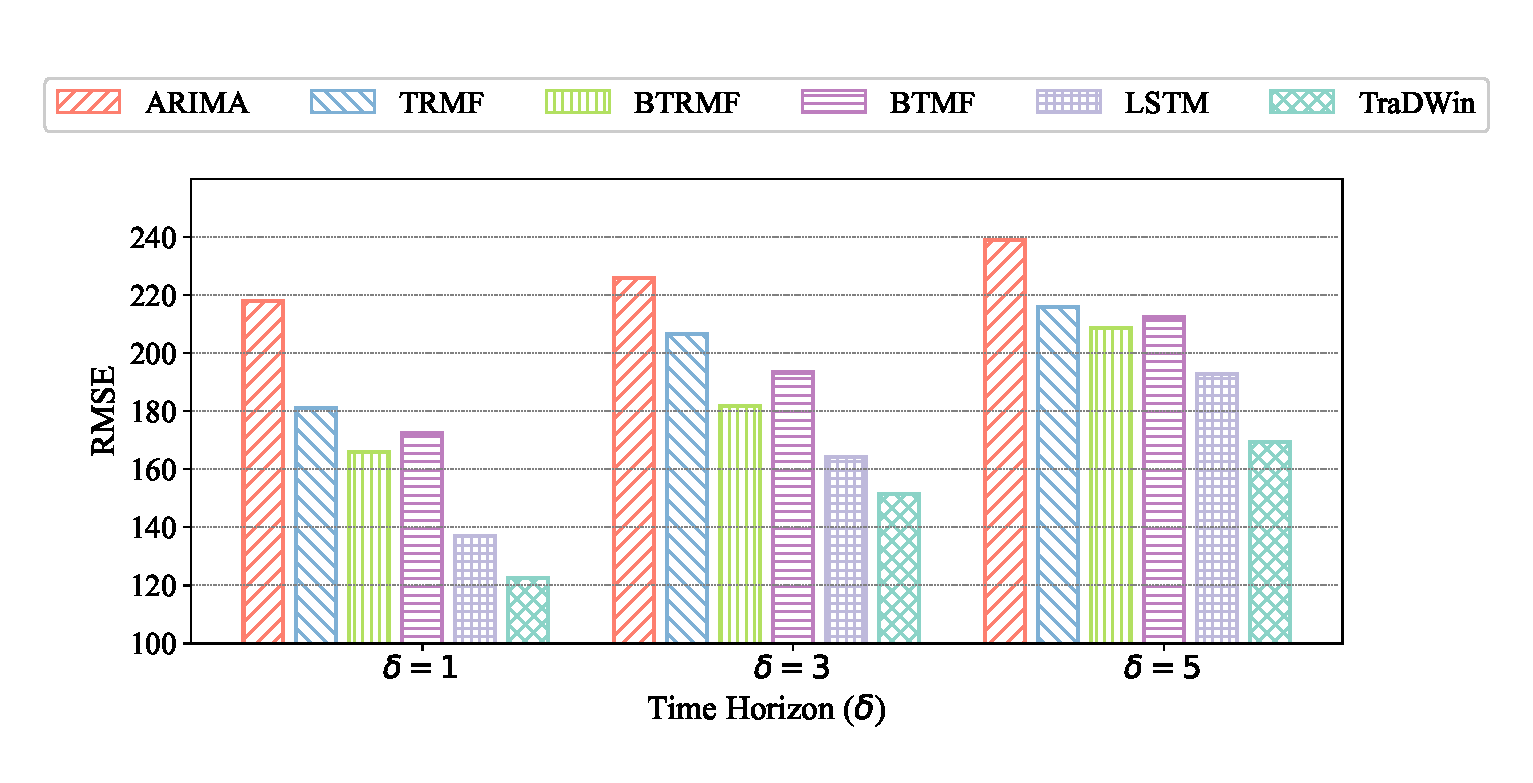
\includegraphics[width=0.9\textwidth]{rmse_pred.eps}
    \caption{RMSE on prediction task for different deltas (timesteps to predict ahead)}
    \label{fig:rmse_pred}
\end{figure*}

We evaluated the performance of our model on different tasks and compared them with other popular models used in the domain. For the prediction task, we tested the models for predicting traffic volumes at the next timestep, i.e., the forecasting $\delta = 1$, at the third timestep, i.e., $\delta = 3$ and the fifth timestep in future, i.e., $\delta = 5$. This scenario of predicting the next time step requires a mask consisting of all the $T_{n+1}$ values missing, i.e., 0. We prepare a mask similarly for other time horizons. Thus, prediction here is treated as a strict MNAR (Missing Not At Random) subcategory of imputation.

The MAPE and RMSE plots of prediction task on different horizons is shown in Fig. \ref{fig:mape_pred} and Fig. \ref{fig:rmse_pred} respectively. We observer that in general, as the $\delta$ i.e. the time horizon to predict in future, increases, both metrics worsen with MAPE falling 5-10\% from $\delta=1$ to $\delta=3$, i.e., we see a stronger short term accuracy but face some challenges with long-term prediction, across all models. This trend is common in time-series forecasting, where predictive accuracy decreases as the prediction horizon extends. The primary reasons for this decline include the increasing uncertainty and the influence of unpredictable external factors, such as accidents or weather changes. We see that ARIMA performs worst, which is to be expected since its the simplest of mathematical models among the baselines we consider. The other matrix factorization and Bayesian models like TRMF, BTRMF and BTMF perform better but given that they are stricly mathematical models, they (i) fail to capture the intricate traffic dynamics that a deep learning model can, and (ii) use only the timeseries traffic data and not the graph topology and external factors that our model considers like weather etc. Finally, we see that LSTMs are close with slightly (2-3\%) worse performance which could be attributed to lack of knowledge of graph topology that we incorporate in our model through $Node2Vec$.

\begin{figure*}[]
  \centering
  \begin{subfigure}{0.5\textwidth}
    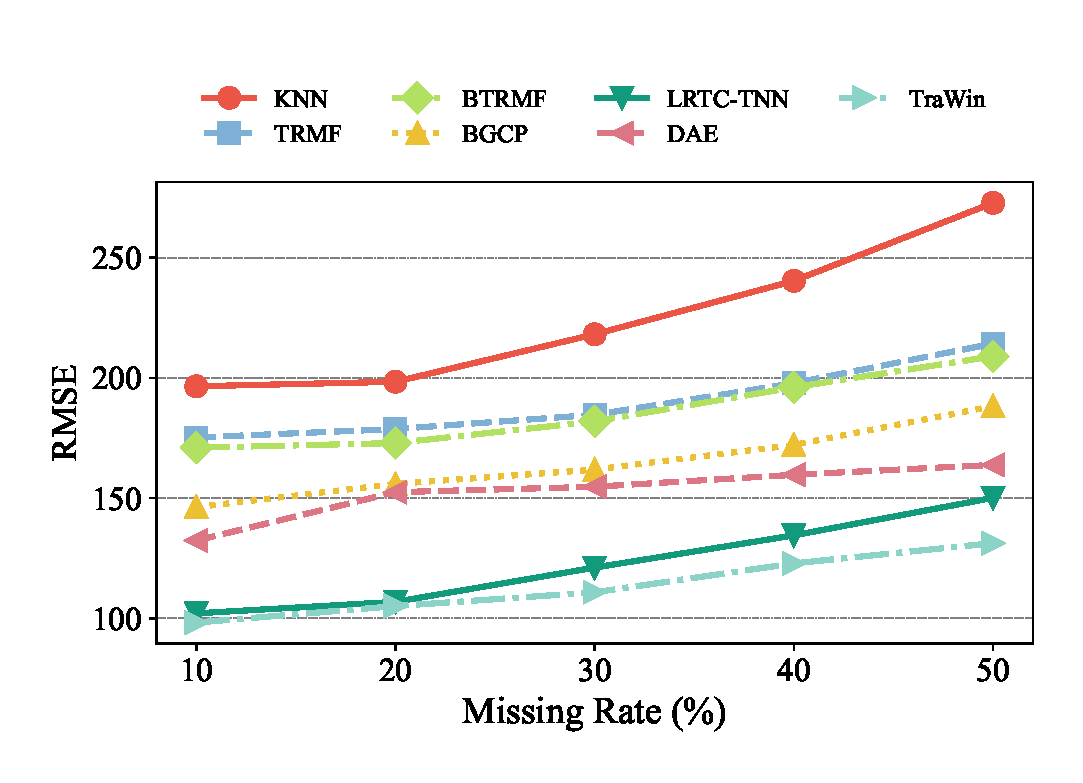
\includegraphics[width=\linewidth]{rmse_imput.eps}
    \caption{RMSE of different models on imputation task}
    \label{fig:mape_imput}
  \end{subfigure}%
  \begin{subfigure}{0.5\textwidth}
    \includegraphics[width=\linewidth]{mape_imput.eps}
    \caption{MAPE of different models on imputation task}
    \label{fig:rmse_imput}
  \end{subfigure}
  \caption{Imputation comparison for different missing rates}
  \label{fig:imput}
\end{figure*}

Next, we evaluate performance on the imptation task. For this task, we have considered the MCAR (Missing Completely At Random) distribution and compare the models at five missing rates of $10\%$, $20\%$, $30\%$, $40\%$ and $50\%$. The perfomance of different models measured using MAPE and RMSE is shown in Fig. \ref{fig:imput}. We see that the conventional methods like KNN, perform poorly to more specialised approaches, which is to be expected since KNN is not enough to capture the intricate traffic dynamics. The matrix factorisation and Bayesian methods which are TRMF, BTRMF and BGCP work slightly better, with deep learning methods like DAE following ahead, though since they deal with only traffic data timeseries with no information on topology they have a 8-13\% worse off performane than out model. Tensor completion based model like LRTC-TNN is close to our \name in for low missing rates, but we see that it does not scale as well with increasing missing rate, possibly because too much data is lost for reliable tensor completion which a deep learning model can still handle, due to being able to learn more complex relationships in data and having knowledge of graph topology and other external factors. Moreover, it is worth nothing that LRTC-TNN is a MCAR imputer and not applicable to task (iii) so not generalised enough for our usecase. For all models, we see that the accuracy of imputations decreases with higher missing rates due to the reduced amount of contextual information available. This is a common challenge in data imputation, where fewer data points make it harder to discern underlying patterns accurately. 


\begin{figure}[t]
    \centering
    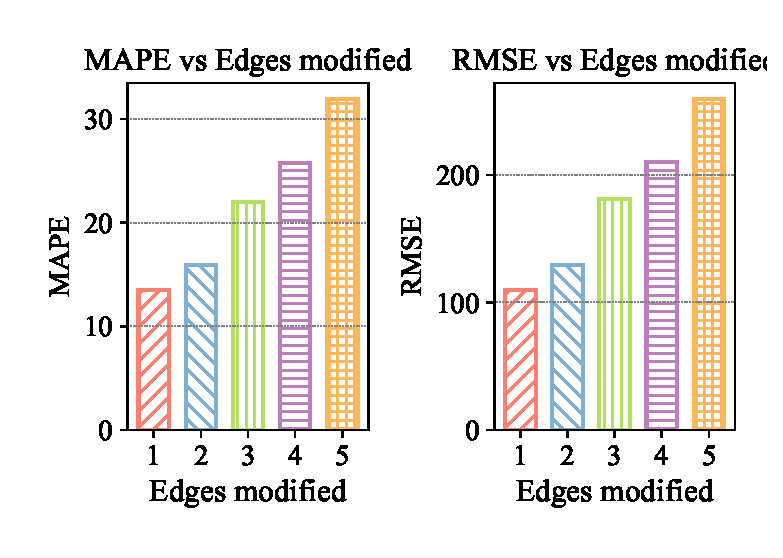
\includegraphics[width=\linewidth]{modif.eps}
    \caption{MAPE and RMSE on re-assignment task vs number of edges modified}
    \label{fig:edge_modif}
\end{figure}

We also observe that \name performs worse on task (i) than task (ii) by around 4\%. One primary reason for this, as we suspect, could be that GAIN that was originally designed for MCAR (Missing Completely At Random) imputation, does not generalise well to MNAR imputation scenarios. Another possible reason could be the subgraph-based computation method that we use, where nodes at the corners of the subgraph do not have adequate spatial and temporal information of their neighbors. Still, we observe that our model performs reasonably and delivers comparable results for being a generalized model.

Finally, on the re-assignment task, which is a new task that we address in our paper and is not conventionally seen in contemporary literature, we essentially train the model for MNAR (Missing Not At Random) imputation scenarios with the central node cluster missing. This effectively makes the model learn how to assign traffic to node clusters given neighbor node information. Based on this training task, we achieve a MAPE of $13.47\%$ and RMSE of $109.90$. Note that the other baselines considered for prediction and imputation are not applicable to this without changes to their model architecture so there is not comparison with contemporary models. Moreover, the de-facto way to solve this problem, as we have seen in our literature review, has been simulations like SUMO\cite{sumo} and Vissim\cite{vissim}. We too use those to compare and test our model on the TAPASCologne scenario using SUMO, which is a traffic simulation engine, with the configuration as described previously. The results of our model on this task are shown in Table. \ref{reassign_table}. We observe that the model achieves a MAPE of $13.47\%$ on Dublin SCATS dataset and $15.06\%$ on the TAPASCologne scenario, which demonstrates that the model can, with reasonable accuracy, learn to solve the traffic assignment problem on node clusters. Further, we tried to evaluate how our model's performance scales with number of modifications, i.e., how much can we alter the original graph such that the model is still viable to use for re-assignment. In Fig. 7, we show a comparison of MAPE and RMSE with number of edges modified. We see that performance declines steadily from $13.47\%$ at $1$ change to $31.91\%$ at 5 changes. So, altering more of graph leads to decline in performance, with drop being significant and sharp after $3$ modifications. A possible reason for this could be the mass masking strategy we use to train the model for task (iii). For 5 modifications, too many of the neighbouring nodes are masked leading to large loss of contextual information that knowledge of graph representation does not compensate enough. 

\section{Conclusion}
In conclusion, we proposed an end-to-end framework, including a model, for an interactive traffic digital twin. We also evaluated and compared our model's performance on the real-world Dublin SCATS dataset, and our experiments showed that the model produced reasonable results compared to other contemporary approaches and techniques in different scenarios. We believe that such a system would be increasingly useful for managing and guiding the decision-making processes related to traffic infrastructure and planning, both by governments and private entities.


\begin{table}[]
\centering
\caption{Performance on re-assignment task (1 edge change) for different datasets}
\label{reassign_table}
\begin{tabular}{lcc}
\toprule
Dataset & MAPE (\%) & RMSE \\
\midrule
Dublin SCATS & 13.47 & 109.90 \\
TAPASCologne & 15.06 & 23.34 \\
\bottomrule
\end{tabular}
\end{table}

\subsection*{Future Work}
It is worth noting that the core architecture of our TDT model is the same for all three underlying tasks. In our approach, we deal with each task as a separate problem for the model to be trained upon. Given that multi-task learning for models, where the model is able to better generalize by learning several different tasks, with output controlled by the parameters of the input itself, has shown promising results, we believe it will be worthwhile to investigate the application of that approach to our model.


\bibliographystyle{IEEEtran}
\bibliography{references}

\end{document}